\documentclass[11pt,a4paper]{report}
\usepackage{amsmath,amssymb,calc,ifthen}
\usepackage{float}
%\usepackage{cancel}
\usepackage[table,usenames,dvipsnames]{xcolor} % for coloured cells in tables
\usepackage{tikz}
% Allows us to click on links and references!
\usepackage{hyperref}
\usepackage{url}
\hypersetup{
colorlinks,
citecolor=black,
filecolor=black,
linkcolor=black,
urlcolor=black
}
% Nice package for plotting graphs
% See excellent guide:
% http://www.tug.org/TUGboat/tb31-1/tb97wright-pgfplots.pdf
\usetikzlibrary{plotmarks,shapes}
\usepackage{amsmath,graphicx}
\usepackage{epstopdf}
\usepackage{caption}
\usepackage{subcaption}
\usepackage{graphicx}
% highlight - useful for TODOs and similar
\usepackage{color}
\newcommand{\hilight}[1]{\colorbox{yellow}{#1}}
\newcommand\ci{\perp\!\!\!\perp} % perpendicular sign
\newcommand*\rfrac[2]{{}^{#1}\!/_{#2}} % diagonal fraction
\newcommand\SLASH{\char`\\}
\usepackage{listings}
% margin size
\usepackage[margin=1in]{geometry}
\usepackage{pdfpages}
\usepackage{enumitem} % for nested enumerate numbers 1 1.1 1.1.1

\usepackage{titlesec} % reduce spacing after subsections

% \titlespacing\subsection{0pt}{4pt plus 4pt minus 2pt}{4pt plus 2pt minus 2pt}


\begin{document}
\belowdisplayskip=12pt plus 3pt minus 9pt
\belowdisplayshortskip=7pt plus 3pt minus 4pt


% Hello dears, 
% 
% Ne pregatim sa facem programul pentru editia de anul acesta a Oxford for Romania. Ma bucur tare mult ca doriti sa va implicati ca lectori sau coordonatori de workshop si sper sa inspiram inca un grup de liceeni impreuna. 
% 
% Ca sa putem sa planificam mai bine, am sa va rog sa trimiteti o scurta propunere de curs pana pe data de 7 august. Nu trebuie sa fie mai mult de un A4, ne-am dori sa atinga urmatoarele puncte: 
% 
% 0. de ce credeti ca ar fi acest curs important pentru elevi
% 1. obiectivele cursului (SMART)
% 2. numarul minim de ore necesare si numarul ideal de ore
% 3. materialele de care aveti nevoie, e.g. proiector, markere, flipchart, internet, sala cu calculatoare si roboti, spaghetti :) s.a.m.d... 
% 4. experienta voastra in teaching (if any)
% 5. intervalul (ele) orare in care ati fi disponibili in perioada 27 aug- 1 septembrie
% 
% Daca ati participat si anul trecut si nu intentionati sa schimbati mare lucru la structura cursului, nu mai este nevoie sa raspundeti la acest email. Pentru cei care nu au participat, trimit cateva exemple de propuneri de anul trecut, poate sunt de ajutor. 
% 
% De asemenea, daca e vreo persoana din lista de lectori cu care considerati ca va puteti grupa (e.g. modulul Medical imaging- Neuroscience de anul trecut), ar fi minunat, pentru ca am asigura continuitatea si o mai buna sustinere a elevilor. 
% 
% Saptamana frumoasa, 


\section*{Aim}

At the end of the course the students will:
\begin{itemize}
 \item Know how 3D computer graphics is used in various industries
 \item Understand the benefits of using computer generated graphics (e.g. saving money) instead of more traditional forms of graphics (e.g. photos, movies)
 \item Know the software available to create 3D computer graphics
 \item Be able to create simple 3D objects
 \item Be able to create a simple animation
 \item Be able to use lightning techniques to create more realistic images
\end{itemize}


\section*{Lesson Plan}

\subsection*{Presentation on 3D computer graphics use in industry - 20 min}

The students will be explained what 3D graphics is and how it is used currently in several industries:
\begin{itemize}
 \item Computer games
 \item Animations 
 \item Special effects in movies
 \item Educational videos (e.g. showing molecular interactions)
 \item Simulations (e.g. car crash tests)
 \item Architecture and interior design
 \item Advertisements
 \item Virtual Reality
\end{itemize}

I will give some examples for each category and explain the motivation for using computer generated graphics in each industry (i.e. save money, generate images not otherwise available in the real world). Finally, I will display some designs I've made in the past, to give the students an idea of what one can do with these skills.

\subsection*{Practical session} 2h

This will be a hands-on session, where I will show the students how to create some basic 3D objects and put them together in a "3D scene". The students will try to replicate my steps as I'm doing them on their computer, and I will pause if any student is left behind. The session will be highly interactive and I will ask students to suggest simple objects which we can then draw together.

Some of the tasks that we will aim to do:
\begin{itemize}
 \item Build a house
 \item Animate the movement of a sailing boat
 \item Build realistic wine glasses with light reflection and refraction
\end{itemize}

\begin{figure}
 \begin{subfigure}{0.3\textwidth}
 \centering
  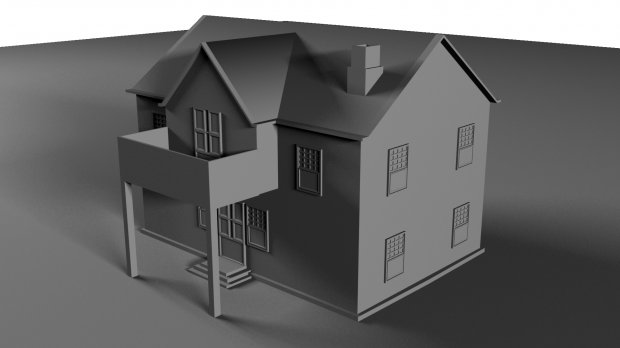
\includegraphics[height=80px]{images/house.jpg}
  \caption{House}
 \end{subfigure}
 \begin{subfigure}{0.3\textwidth}
 \centering
  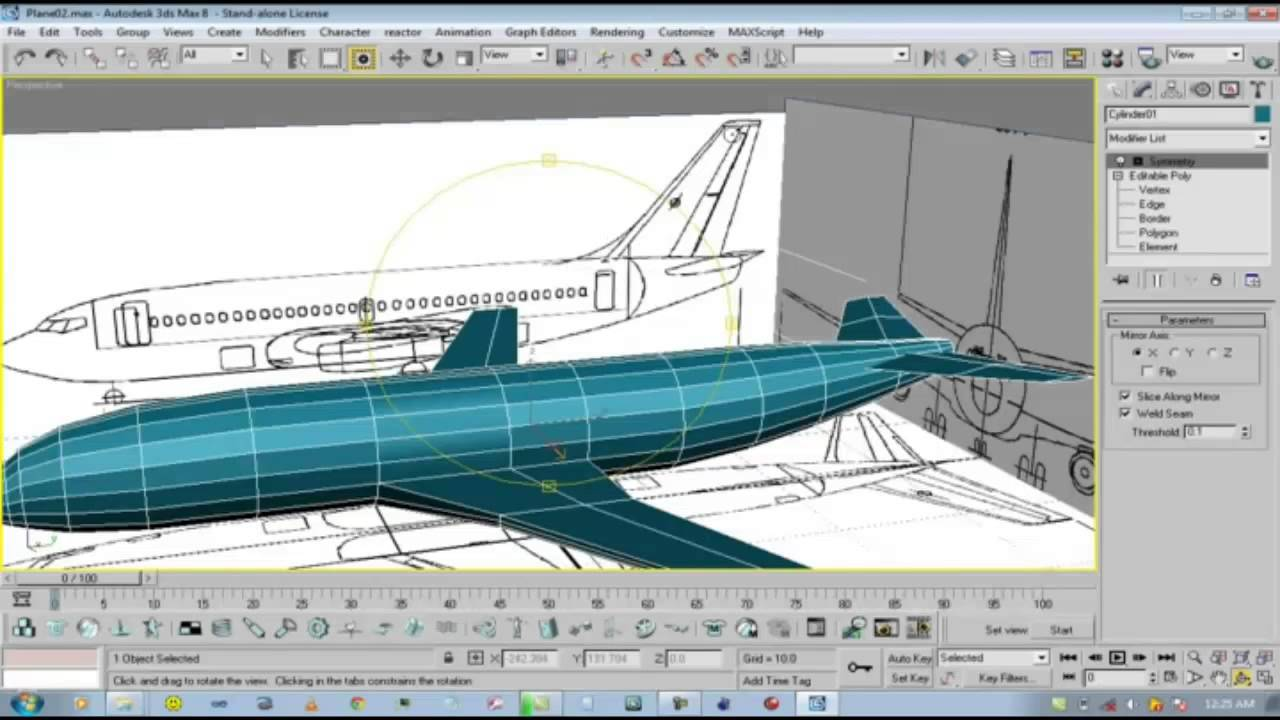
\includegraphics[height=80px, trim=0 0 200 0, clip]{images/plane.jpg}
  \caption{Plane}
 \end{subfigure}
 \begin{subfigure}{0.3\textwidth}
 \centering
  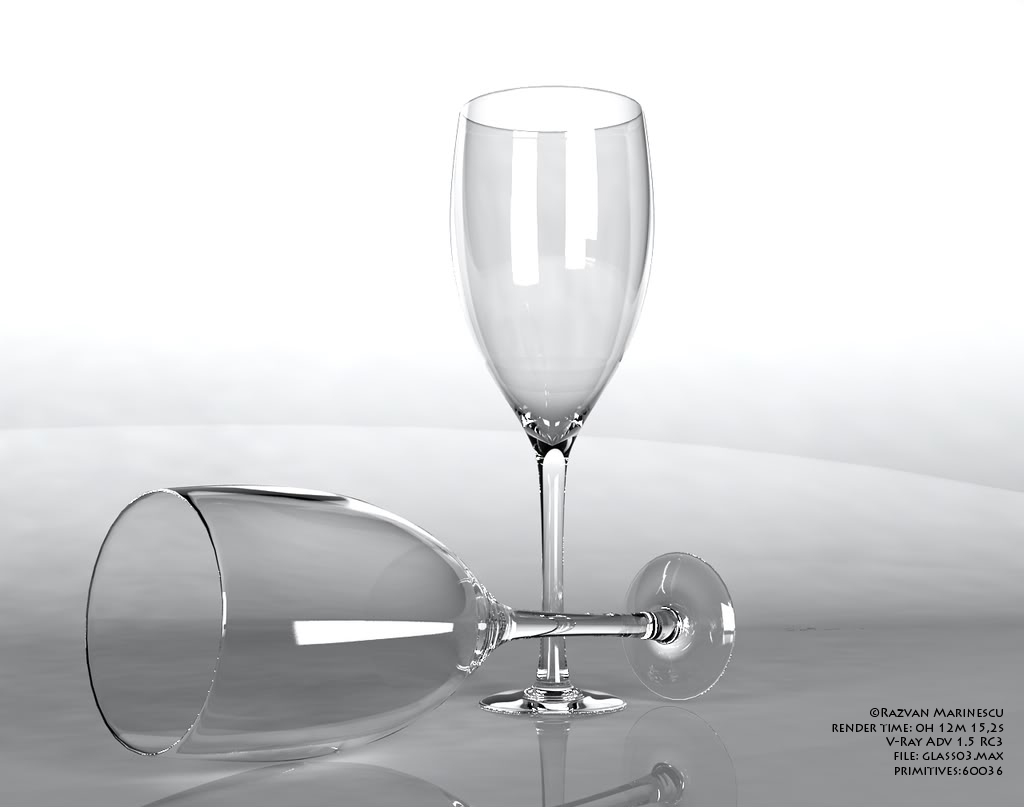
\includegraphics[height=80px]{images/glass03.jpg}
  \caption{Realistic wine glasses}
 \end{subfigure}
\end{figure}



\subsection*{Creativity session} - 1h

The students will be grouped into teams and each team will be free to draw anything they like. At the end of the session, the teams will display their 3D images/animations in front of everyone else. Everyone will vote for the best 3D object/animation (self voting not permitted) and the winner team will be awarded a prize.


\section*{Teaching experience}

I have organised a 3-week course on this topic in 2013 at Imperial College (IC) London. I have also been a tutor for several programming and modelling courses:
\begin{itemize}
 \item Programming in Java/C++: Taught this for 1.5 years to first-year undergraduate students at IC
 \item Computational Modelling in Medical Imaging: Taught this for 
\end{itemize}


\section*{Personal portofolio}

\begin{figure}[H]
 \begin{subfigure}{0.47\textwidth}
 \centering
 \vspace{1em}
  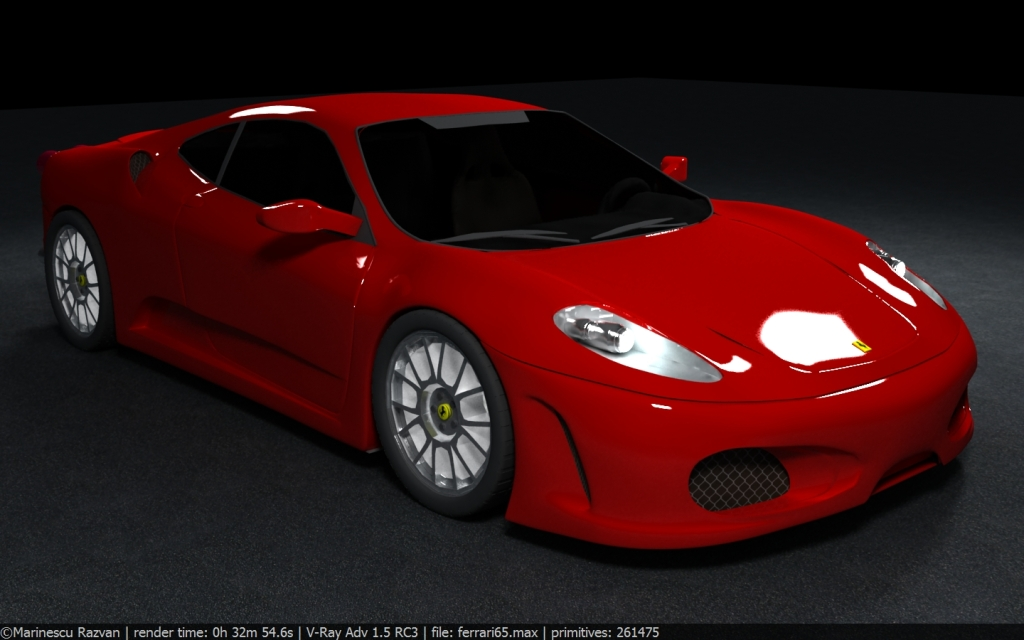
\includegraphics[width=\textwidth]{images/ferrari1440x900.jpg}
 \end{subfigure}
 \begin{subfigure}{0.47\textwidth}
 \centering
  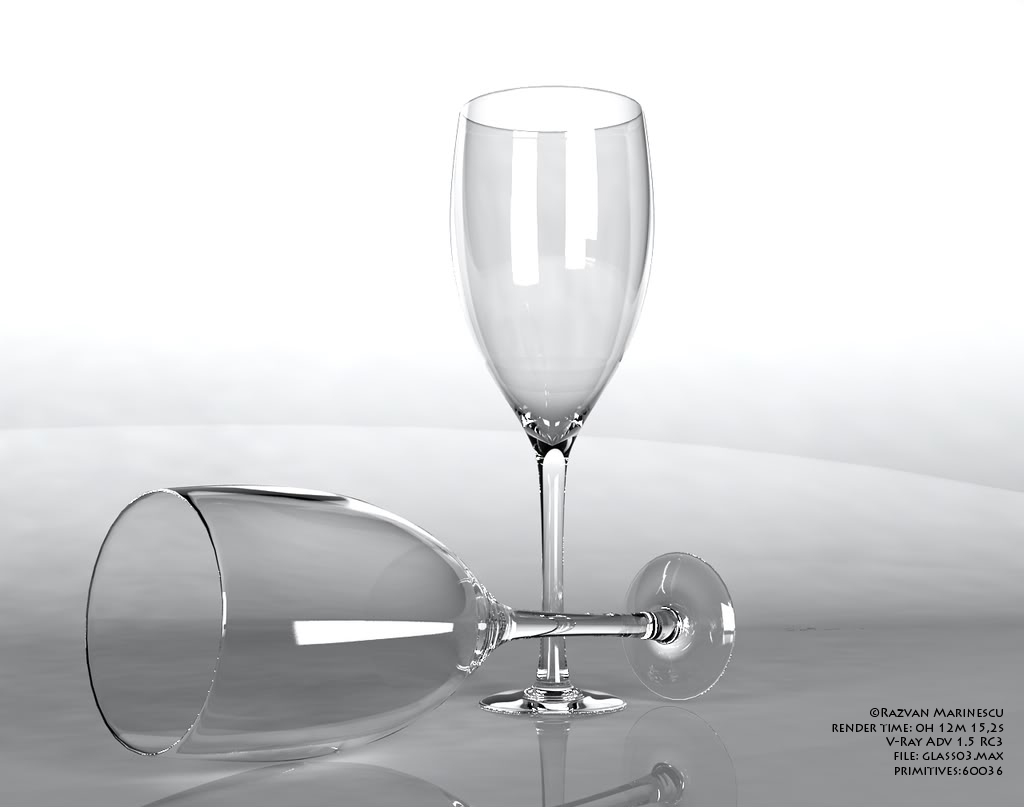
\includegraphics[width=\textwidth]{images/glass03.jpg}
 \end{subfigure}
 
 \begin{subfigure}{0.47\textwidth}
 \centering
  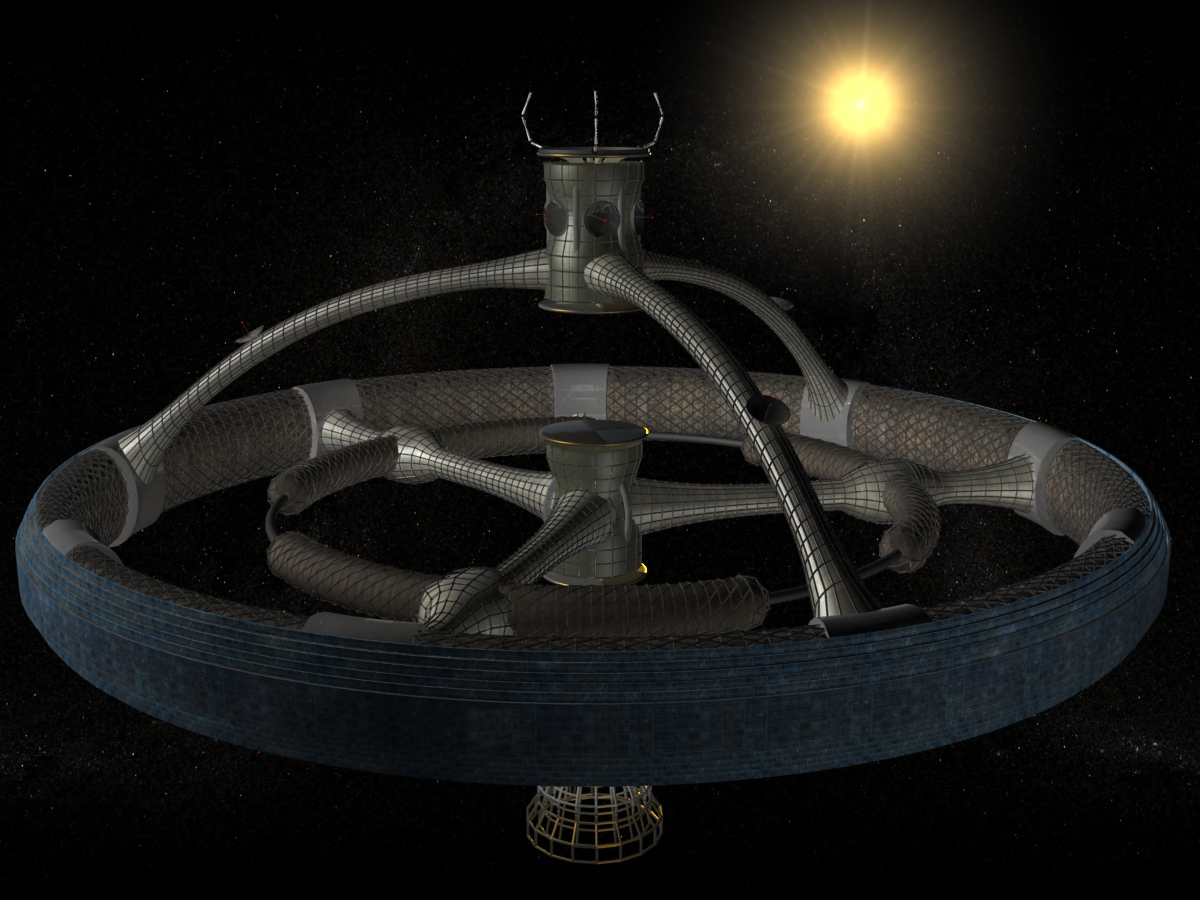
\includegraphics[width=\textwidth]{images/station02}
 \end{subfigure}
 \begin{subfigure}{0.47\textwidth}
 \centering
  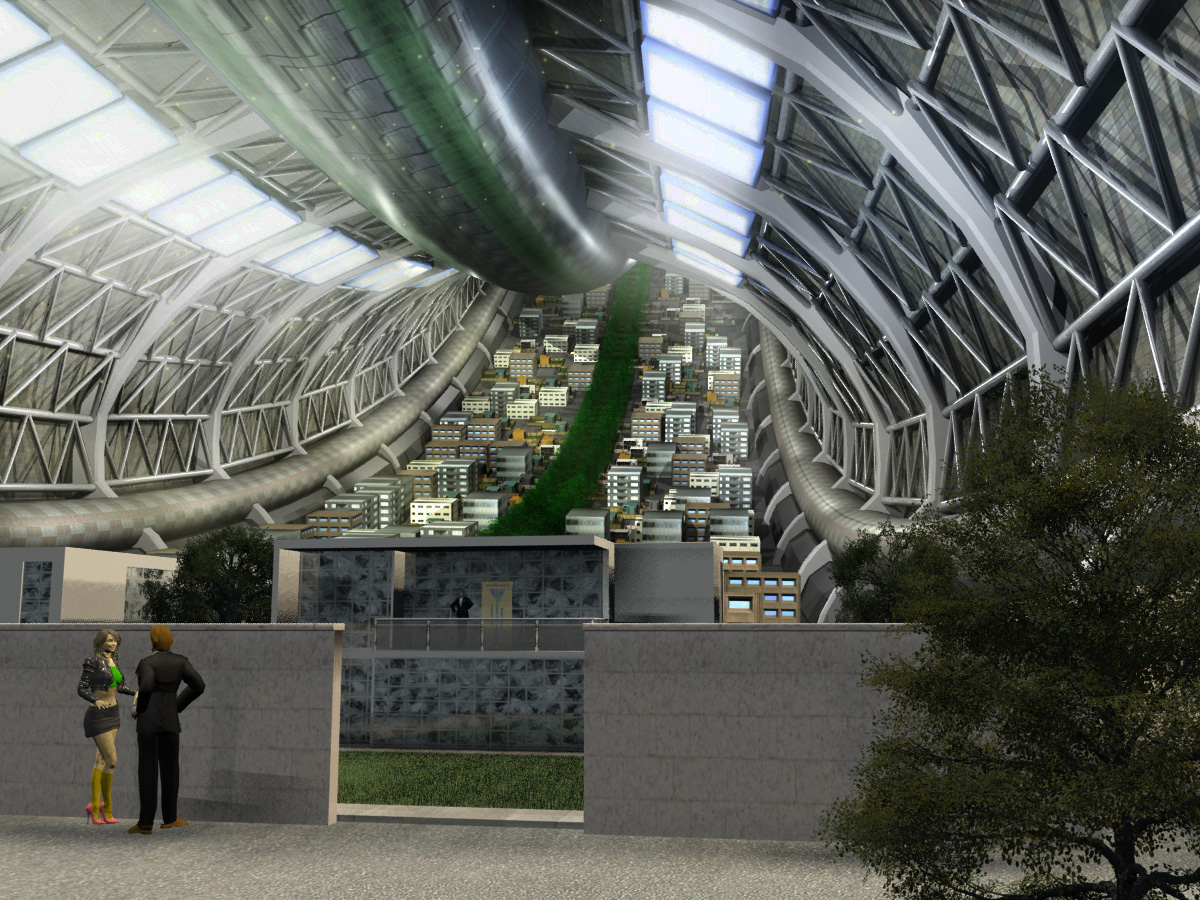
\includegraphics[width=\textwidth]{images/interior-final}
 \end{subfigure}
 
 \begin{subfigure}{0.47\textwidth}
 \centering
  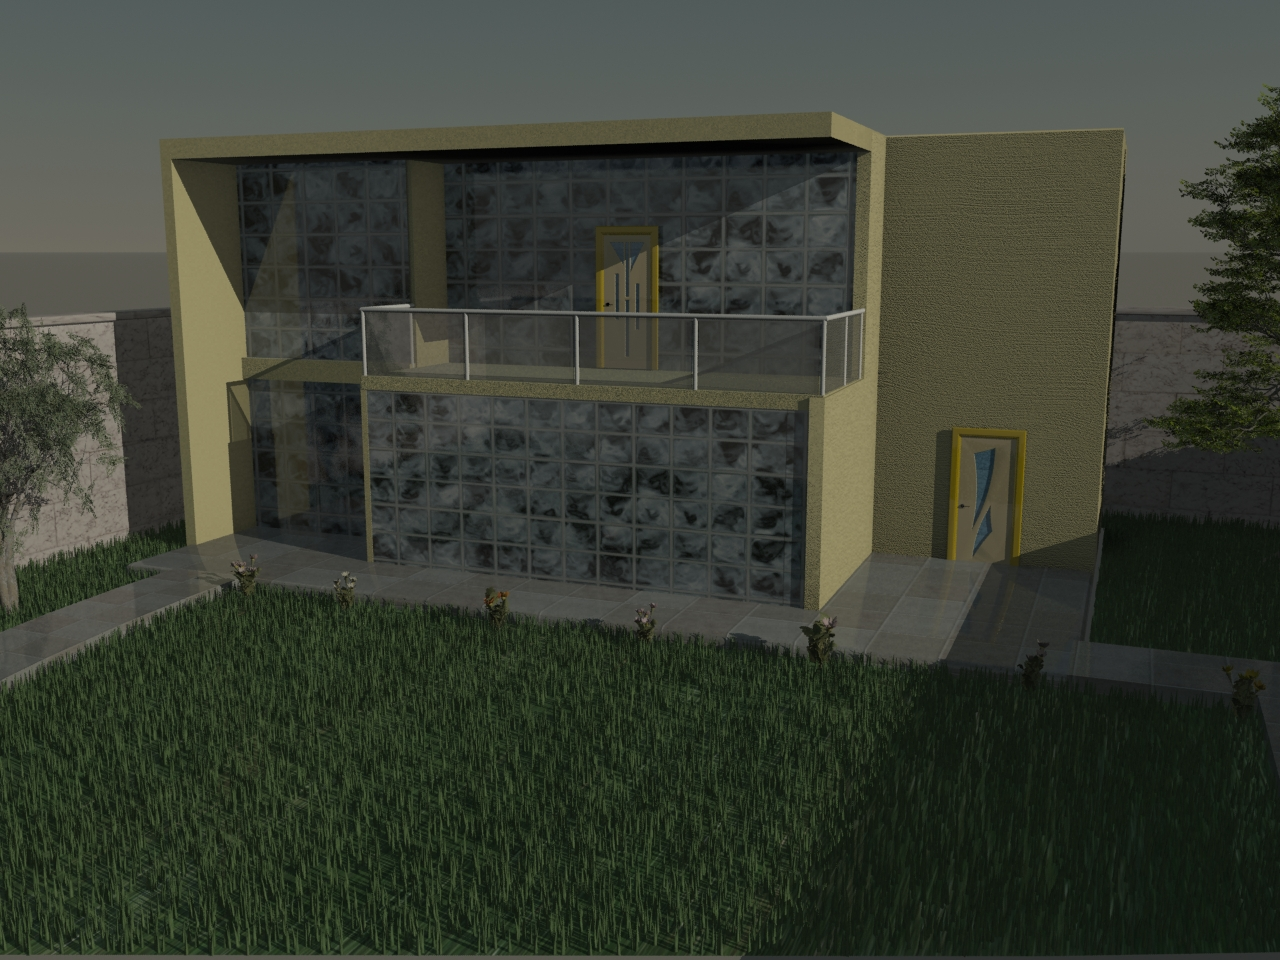
\includegraphics[width=\textwidth]{images/house2}
 \end{subfigure}
 
 
 
 \caption{Collage of 3D computer-generated images that I've done so far.}
\end{figure}




\section*{Availability}




\end{document}





















